\title [概率论]{第八讲:随机变量及其分布}
%\author [张鑫 {\rm Email: x.zhang.seu@foxmail.com} ]{\large 张 鑫}
\institute [东南大学数学学院]{\large \textrm{Email: xzhangseu@seu.edu.cn} \\ \quad  \\
	\large 东南大学 \quad 数学学院 \\
	\vspace{0.3cm}
	%  \trc{公共邮箱: \textrm{zy.prob@qq.com}\\
	%    \hspace{-1.7cm}  密 \qquad 码: \textrm{seu!prob}}
}
\date{}



{ \setbeamertemplate{footline}{}
	\begin{frame}
		\titlepage
	\end{frame}
}

% \begin{frame}[plain]
%   \frametitle{目录}
%   \setcounter{tocdepth}{2}
%   \tableofcontents
% \end{frame}
\addtocounter{framenumber}{-3}  % 目录页不计算页码
\section{随机变量}

\subsection{随机变量的定义及性质}


\begin{frame}{随机变量的引入}
	\begin{itemize}[<+-|alert@+>]
		\item 赌徒输光:甲和乙初始资金分别为 $i, a-i$ 元,每一局甲赢的概率为 $p$%\in (0,1)$.
		\item 关注的问题
		      \begin{itemize}[<+-|alert@+>]
			      \item 甲最终获胜的概率
			      \item 甲乙两人在任意时刻的剩余资产:$k$ 轮赌博后恰好剩下 $j$ 元
			      \item $k$ 轮赌博后甲乙两人资产的差额 $Z$
			      \item 赌博持续时间 $R$
		      \end{itemize}
		\item 表示方法:
		      \begin{itemize}[<+-|alert@+>]
			      \item $E:=$\{甲最终获胜 \}, $Q_i:=P$(E)
			      \item $A_{jk}:=$\{甲在 $k$ 轮赌博后恰好剩下 $j$ 元 \}
			      \item $B_{jk}:=$\{乙在 $k$ 轮赌博后恰好剩下 $j$ 元 \}
			      \item $k$ 轮赌博后甲乙两人资产的差额如何表示?
			      \item 赌博持续时间 $R$ 如何表示?
			      \item 很难用事件来表示或者表示很复杂
		      \end{itemize}

	\end{itemize}

\end{frame}

\begin{frame}{随机变量的引入}
	\begin{itemize}[<+-|alert@+>]
		\item $X_k:=$ 甲在 $k$ 轮赌博后的资产
		      \begin{itemize}[<+-|alert@+>]
			      \item 乙在 $k$ 轮赌博后的资产 $Y_k=a-X_k$
			      \item 资产差额:$Z=X_k-Y_k=2X_k-a$
			      \item 持续时间:$R=\min\{n: X_n=0, \mbox{或} Y_n=0\}$
		      \end{itemize}
		\item $X_k$ 取值的特点
		      \begin{itemize}[<+-|alert@+>]
			      \item 依赖于前面 $k$ 次赌博这一 “随机试验” 的结果
			      \item 在 “随机试验” 完成之前,$X_k$ 取值不确定,因此具有不确定性
			      \item $k$ 次赌博 “随机试验” 一旦完成,$X_k$ 的值必然确定
			      \item 记 $k$ 次赌博 “随机试验” 样本空间为 $\Omega$, 则给定 $\omega\in\Omega$, 则 $X_k$ 值确定
		      \end{itemize}
		\item 以 $k=2$ 为例,看一下 $X_2$ 的取值情况,设 $i\geq 2$
		      \begin{itemize}[<+-|alert@+>]
			      \item $\Omega=\{\omega_1,\omega_2, \omega_3,\omega_4\}$, 其中 $\omega_1=(\mbox{胜,胜}), \omega_2=(\mbox{胜,败}), \omega_1=(\mbox{败,胜}), \omega_1=(\mbox{败,败})$
			      \item $X_2(\omega_1)=i+2,\  X_2(\omega_2)=X_2(\omega_3)=i,\  X_2(\omega_4)=i-2$
		      \end{itemize}
		\item $X_k$ 可以看作定义在样本空间 $\Omega$ 上的函数,即 $X_k:\Omega\rightarrow \{0, 1,\cdots, a\}$
		\item 一般的,随机变量可以看作从样本空间到实数的映射:$X:\Omega\rightarrow R$

	\end{itemize}

\end{frame}
\begin{frame}{随机变量的直观定义}
	\begin{defi} \textcolor{cyan}{(直观定义)}
		称 $X$ 为随机变量,如果 $X$ 是从样本空间 $\Omega$ 到实数的映射,即 $X:\Omega\rightarrow R$.
	\end{defi}

\end{frame}
\begin{frame}{一个随机变量的例子}
	\begin{exam}\label{312}
		考虑硬币抛掷两次的随机试验,其样本空间为 $$\Omega=\{HH,HT,TH,TT\}.$$ % 这里存在该空间上的一些随机变量 (用于实践,你也可以想出一些自己的随机变量). 每一个随机变量都是试验在某方面的数值表示.%
		\begin{itemize}[<+-|alert@+>]
			\item 令 $X$ 表示正面朝上的次数,则 $X$ 是一个随机变量,相应的映射如下
			      % 其可能的取值为 0、1、2. 将其看作是一个函数,$X$ 作用在 $HH$ 上的值为 2,$X$ 作用在 $TH$ 或者 $HT$ 上的值为 1,$X$ 作用在 $TT$ 上的值为 0, 即
			      $$X(TT)=0, X(HT)=X(TH)=1, X(HH)=2.$$
			\item 令 $Y$ 表示反面朝上的次数,则 $Y=2-X$, 对于任意的 $\omega\in \Omega$, 有 $Y (\omega)=2-X (\omega)$.
			\item 设 $I$ 是由第一次掷硬币的结果决定的随机变量:若第一次硬币正面朝上则 $I=1$, 反之 $I=0$, 即
			      \begin{align*}
				      I(HH)=I(HT)=1,\quad I(TH)=I(TT)=0.
			      \end{align*}
			\item 若正面记 1, 反面记 0, 此时 $\Omega=\{(1,1),(1,0),(0,1),(0,0)\}$. 上述的 $X,Y$ 和 $I$ 可表示为:$$X (\omega_1,\omega_2)=\omega_1+\omega_2,Y (\omega_1,\omega_2)=2-\omega_1-\omega_2,I (\omega_1,\omega_2)=\omega_1.$$
		\end{itemize}
	\end{exam}
\end{frame}


\begin{frame}{与函数对比分析}
	\begin{itemize}[<+-|alert@+>]
		\item 数学分析中的函数 $f (x)$
		      \begin{itemize}[<+-|alert@+>]
			      \item $f (x):D\rightarrow R$, 其中 $D\subset R$
			      \item $R$ 上可定义距离 $d (x,y)=|x-y|$
			      \item 可根据距离 $d$ 定义函数的连续性 %
		      \end{itemize}
		\item 概率论中的随机变量 $X$
		      \begin{itemize}[<+-|alert@+>]
			      \item $X(\omega):\Omega\rightarrow R$
			      \item 定义域 $\Omega$ 没有距离的定义,\pause 但有事件域 $\mathcal{F}$ 及定义其上的概率 $P$, 即具有结构 $(\Omega, \mathcal{F}, P)$\pause
			      \item 值域 $R$ 有距离,\pause 但因定义域无距离,故无法考虑随机变量的连续性 \pause
			      \item 值域 $R$ 还有 $\sigma$- 代数 $\mathcal{B}:=\mathcal{B}(R)$, 有可测空间结构 $(R,\mathcal{B})$
		      \end{itemize}
		\item 是否需要对 $X (\omega):\Omega\rightarrow R$ 做一些额外的限定,以便更好的研究 $X$?
		\item 从赌徒输光问题可以看出,对随机变量 $X$, 我们会关注
		      \begin{itemize}[<+-|alert@+>]
			      \item $X (\omega)=x$ 的概率,\pause $X (\omega)\leq x, X (\omega)\in [b,c]$ 的概率 \pause
			      \item 更一般的,$\forall B\in\mathcal{B}(R), X (\omega)\in B$ 的概率
		      \end{itemize}
		\item 概率的定义域是 $\mathcal{F}$, 要想计算 $X (\omega)\in B$ 的概率,当且仅当
		      \[\forall B\in\mathcal{B}(R), \ X^{-1}(B):=\{\omega: X(\omega)\in B\}\in\mathcal{F}\]
	\end{itemize}
\end{frame}






\begin{frame}
	\frametitle{随机变量的严格数学定义}
	\vspace{-0.1cm}
	\begin{defi}[可测映射] 设 $(\Omega,\mathcal{F})$ 和 $(E,\mathcal{E})$ 为两个可测空间并令 $X$ 为从样本空间 $\Omega$ 到 $E$ 的映射,即 $X (\omega):\Omega\rightarrow E$. 若对任意的 $B\in \mathcal{E}$ 均有
		\begin{eqnarray*}
			X^{-1}(B):=\{\omega: X(\omega)\in B\}\in \mathcal{F}
		\end{eqnarray*}
		则称 $X$ 为 $(\Omega,\mathcal{F})$ 到 $(E,\mathcal{E})$ 的可测映射.
	\end{defi}
	\pause %

	若将上述定义中的可测空间 $(E,\mathcal{E})$ 更换为 $(R,\mathcal{B})$,则 % 所定义的可测映射称为可测空间 $(\Omega,\mathcal{F})$ 上的可测函数或随机变量,即:
	\pause
	\begin{defi}[可测函数或随机变量] \label{rvdefi1}\hspace{-0.2cm} 设 $(\Omega,\mathcal{F})$ 是可测空间,$X$ 为从样本空间 $\Omega$ 到实数集 $R$ 的映射,即 $X (\omega):\Omega\rightarrow R$. 如果对 $\forall B\in \mathcal{B}$ 均有
		\[X^{-1}(B):=\{\omega: X(\omega)\in B\}\in \mathcal{F}.\]%
		则称 $X$ 为可测空间 $(\Omega,\mathcal{F})$ 上的可测函数或随机变量.
	\end{defi}%
	\pause
	\begin{defi}[随机变量的另一定义]\hspace{-0.2cm} \label{rvdefi2} 设 $(\Omega,\mathcal{F})$ 是可测空间,$X$ 为从样本空间 $\Omega$ 到实数集 $R$ 的映射,即 $X (\omega):\Omega\rightarrow R$. 如果对任意的 $x\in R$ 均有
		\begin{eqnarray*}
			\{\omega: X (\omega)\le x\}\in \mathcal{F} \mbox{  或  }      \{\omega: X (\omega)< x\}\in \mathcal{F}
		\end{eqnarray*}
		则称 $X (\omega)$ 是可测空间 $(\Omega,\mathcal{F})$ 上的随机变量,简称随机变量.
	\end{defi}
\end{frame}
\begin{frame}
	\frametitle{随机变量两种定义的等价性}
	由定义 \ref{rvdefi2} 推定义 \ref{rvdefi1}: 仅需说明若定义 \ref{rvdefi2} 成立,则对任意 $B\in\mathcal{B}$ 均有
	$$X^{-1}(B):=\{\omega:X(\omega)\in B\}\in \mathcal{F}.$$
	\pause 即只需说明以下集合包含关系成立即可
	\begin{eqnarray*}
		\mathcal{A}:=\{A:X^{-1}(A)\in \mathcal{F}\}\supset \mathcal{B}
	\end{eqnarray*}
	\pause
	欲证上面包含关系成立,我们只需说明以下两点即可:
	\begin{enumerate}[<+-|alert@+>]
		\item $\mathcal{A}$ 是 $\sigma$ 代数;
		\item $O_1:=\{(-\infty,x]:x\in R\}\subset \mathcal{A}$.
	\end{enumerate}
	\pause 再由 $\mathcal{B}:=\sigma (O_1)$ 知 $\mathcal{B}\subset \mathcal{A}$.
\end{frame}
\begin{frame}
	\frametitle{$\mathcal{A}:=\{A:X^{-1}(A)\in \mathcal{F}\}$ 为 $\sigma$ 代数}
	\begin{itemize}[<+-|alert@+>]
		\item $X^{-1}(R)=\{\omega:X (\omega)\in R\}=\Omega\in \mathcal{F}$, 故 $R\in\mathcal{A}$;
		\item 若 $A\in\mathcal{A}$, 即 $X^{-1}(A)\in \mathcal{F}$, 则
		      \begin{eqnarray*}
			      X^{-1}(\overline{A})&=&\pause \{\omega: X(\omega)\in \overline{A}\}\pause =\{\omega:X(\omega)\notin A\}\\
			      &=&\pause \overline{\{\omega:X(\omega)\in A\}}=\pause \overline{X^{-1}(A)}\\ \pause &\in&  \mathcal{F}
		      \end{eqnarray*}
		\item 对于 $A_j\in \mathcal{A}, j=1,2,\cdots,$ 有 $X^{-1}(A_j)\in \mathcal{F},j=1,2,\cdots.$ 从而
		      \begin{eqnarray*}
			      X^{-1}(\cup_{j=1}^\infty A_j)&=&\pause \{\omega:X(\omega)\in\cup_{j=1}^\infty A_j\}
			      =\pause \cup_{j=1}^\infty \{\omega:X(\omega)\in A_j\}\\
			      &=&\pause \cup_{j=1}^\infty X^{-1}(A_j)\\ \pause &\in&\mathcal{F}
		      \end{eqnarray*}

	\end{itemize}
\end{frame}

\begin{frame}{随机变量的分类}
	\begin{itemize}[<+-|alert@+>]
		\item 随机变量 $X$ 是从样本空间 $\Omega$ 到实数 $R$ 的映射,故根据其值域集合可粗略的分为两大类
		      \begin{itemize}[<+-|alert@+>]
			      \item 离散型随机变量:其值域集合是有限点集或可数点集即
			            \[X(\Omega):=\{X(\omega):\omega\in \Omega\}=\{a_n\}_{n\geq 1}\]
			      \item 非离散型随机变量:其值域集合不是有限点集或可数点集
		      \end{itemize}
	\end{itemize}
\end{frame}


\begin{frame}{示性随机变量}
	\begin{exam}
		设 $\Omega$ 是某随机试验的样本空间,$\mathcal{F}$ 为其事件域 ($\sigma$ 代数),则对于任意的 $A\in \mathcal{F}$, 示性函数
		$I_A(\omega):=\left\{
			\begin{array}{ll}
				0, & \omega\notin A \\
				1, & \omega\in A
			\end{array}\right.$ 是随机变量.
	\end{exam}

	\pause
	\jieda  由示性函数的定义知:
	\begin{eqnarray*}
		\{\omega:I_A(\omega)\le x\}=\left\{
		\begin{array}{ll}
			\pause \emptyset, & x<0,        \\ \pause
			\overline{A},     & x\in [0,1), \\\pause
			\Omega,           & x\ge 1.
		\end{array}
		\right.
	\end{eqnarray*}
	\pause
	显然,无论 $x$ 取何值,均有 $\{\omega:I_A (\omega)\le x\}\in \mathcal{F}$


\end{frame}





\begin{frame}
	\frametitle{随机变量的性质}
	\begin{thm}
		若 $X,Y, \{X_n,n\ge 1\}$ 都为概率空间 $(\Omega,\mathcal{F},P)$ 上的随机变量,则
		\begin{enumerate}[<+-|alert@+>]
			\item $|X|$,$aX+bY,(a,b\in R)$ 均为随机变量;
			\item $X^+:=X\vee 0, X^-:=(-X)\vee 0$ 均为随机变量;
			\item $XY$ 为随机变量;
			\item 若 $X/Y$ 处处有意义,则 $X/Y$ 为随机变量;
			\item $\inf_{n} X_n,\sup_nX_n, \liminf_{n\rightarrow\infty} X_n, \limsup_{n\rightarrow\infty} X_n$ 均为随机变量.
		\end{enumerate}

	\end{thm}

	\pause
	\zheng
	\begin{enumerate}[<+-|alert@+>]
		\item
		      \begin{itemize}[<+-|alert@+>]
			      \item $\{\omega:|X|<x\}=\{\omega:-x<X<x\}=\{\omega:X<x\}\cap\overline{\{\omega:X\le -x\}}\in \mathcal{F}$;
			      \item  $\{\omega:aX<x\}=\{\omega:X<\dfrac{x}{a}\}\in \mathcal{F}$,  (当 $a>0$ 时);
			      \item  设 $Q$ 为有理数集,则
			            \begin{eqnarray*}
				            \{\omega:X+Y<x\}&=&\pause \{\omega:X<x-Y\}=\pause \cup_{r\in Q}\{\omega:X<r<x-Y\}\\
				            &=&\pause \cup_{r\in Q}\{\omega:X<r,Y<x-r\}\\
				            &=&\pause \cup_{r\in Q}(\{\omega:X<r\}\cap \{\omega:Y<x-r\})\\\pause
				            &\in& \mathcal{F}
			            \end{eqnarray*}
			      \item $aX+bY$ 为随机变量显然
		      \end{itemize}
	\end{enumerate}


\end{frame}
\begin{frame}
	\vspace{0.6cm}
	\begin{enumerate}[<+-|alert@+>]
		\setcounter{enumi}{1}
		\item 注意到 $X^+=\dfrac{|X|+X}{2}, X^-=\dfrac{|X|-X}{2}$,易得 $X^+,X^-$ 均为随机变量;
		\item 首先假定 $X,Y$ 非负, 则对任意的 $x>0$ 有
		      \begin{eqnarray*}
			      \{XY<x\}&=&\pause \{X=0\}\cup \{Y=0\}\cup \left(\cup_{r\in Q_+}\left[\{X<r\}\cap \{Y<\frac{x}{r}\}\right]\right)\\ \pause
			      &\in&\mathcal{F}.
		      \end{eqnarray*}
		      \pause
		      对一般的 $X,Y$, 由 $X^+,X^-,Y^+,Y^-$ 为随机变量,可得
		      \begin{eqnarray*}
			      XY=(X^+-X^-)(Y^+-Y^-)=(X^+Y^++X^-Y^-)-(X^+Y^-+X^-Y^+)
		      \end{eqnarray*}
		      为随机变量.
		\item 设 $|Y|>0$ 处处成立,易证 $\dfrac{1}{Y}$ 是随机变量, 故 $\dfrac{X}{Y}=X\cdot \dfrac{1}{Y}$ 为随机变量.
		\item 对任意的 $x\in R$, 我们有
		      \begin{eqnarray*}
			      \{\inf_nX_n<x\}=\cup_n\{X_n<x\}, \quad \{\sup_nX_n\le x\}=\cap_n\{X_n\le x\}
		      \end{eqnarray*}

	\end{enumerate}


\end{frame}

\begin{frame}
	\frametitle{简单随机变量}
	\begin{exam}
		设 $(\Omega,\mathcal{F},P)$ 为一概率空间,$A_i\in\mathcal{F}, i=1,\cdots,n$ 为 $\Omega$ 的一个分割,$a_i,i=1,\cdots, n$ 为 $n$ 个不同的实数,则
		\begin{eqnarray}\label{eq:simplerv}
			X(\omega):=\sum_{i=1}^na_iI_{A_i}(\omega)
		\end{eqnarray}
		作为 $n$ 个示性随机变量的线性组合,仍为随机变量。我们称形如 \eqref{eq:simplerv} 的 $X (\omega)$ 为简单随机变量.
	\end{exam}

\end{frame}

\begin{frame}{随机变量的函数是否仍为随机变量?}
	\vspace{0.5cm}
	\begin{thm}
		设 $X$ 是可测空间 $(\Omega,\mathcal{F})$ 上的随机变量,$g (x)$ 为 $(R,\mathcal{B})\rightarrow (R,\mathcal{B})$ 上的可测函数,证 $Y:=g (X)$ 为 $(\Omega,\mathcal{F})$ 上的随机变量.
	\end{thm}

	\vspace{0.3cm}
	\pause
	\jieda 注意到,对任意的 $B\in \mathcal{B}$, $g^{-1}(B)\in \mathcal{B}$, 故 \pause
	\begin{align*}
		Y^{-1}(B) & =\pause \{\omega:Y(\omega)\in B\}         \\
		          & =\pause \{\omega:g(X(\omega))\in B\}      \\
		          & =\pause \{\omega:X(\omega)\in g^{-1}(B)\} \\
		          & =\pause X^{-1}(g^{-1}(B))                 \\ \pause
		          & \in  \mathcal{F}
	\end{align*}

\end{frame}


\begin{frame}
	\frametitle{随机变量的结构}
	对于 $(\Omega,\mathcal{F},P)$ 上的任意非负随机变量 $X$ 及自然数 $n$,我们可将 $\Omega$ 按 $X$ 的取值进行分割。即令
	\begin{eqnarray*}
		A_k(\omega)&:=&\pause \{\omega:\frac{k}{2^n}\le X(\omega)<\frac{k+1}{2^n}\}, k=0,1,\cdots, n2^n-1\\
		A_{n2^n}(\omega)&:=&\pause \{\omega:X(\omega)\ge n\}
	\end{eqnarray*}
	\pause 则
	\begin{eqnarray*}
		X_n(\omega):=\sum_{k=0}^{n2^n}\frac{k}{2^n}I_{A_k}(\omega)
	\end{eqnarray*}
	为简单随机变量且随机变量序列 $\{X_n,n\ge 1\}$ 满足
	\begin{eqnarray*}
		0\le X_1(\omega)\le X_2(\omega)\le \cdots\le X_n(\omega)\rightarrow X(\omega)
	\end{eqnarray*}
\end{frame}
\begin{frame}
	\frametitle{$X_n (\omega)$ 的单调性}
	% 事实上,要说明 $X_n (\omega)\le X_{n+1}(\omega)$,只需要说明在 $\Omega$ 有限分割集合 $A_k, k=0,1,\cdots,n2^n$ 上均有 $X_n (\omega)\le X_{n+1}(\omega)$.
	注意到对任意的 $k=0,1,\cdots,n2^n-1$,
	\begin{eqnarray*}
		A_k(\omega)&=&\pause \{\omega:\frac{k}{2^n}\le X(\omega)<\frac{k+1}{2^n}\}=\pause \{\omega:\frac{2k}{2^{n+1}}\le X(\omega)<\frac{2(k+1)}{2^{n+1}}\}\\
		&=&\pause \{\omega:\frac{2k}{2^{n+1}}\le X(\omega)<\frac{2k+1}{2^{n+1}}\}\cup \{\omega:\frac{2k+1}{2^{n+1}}\le X(\omega)<\frac{2k+2)}{2^{n+1}}\}\\
		&=&\pause A_k^1(\omega)\cup A_k^2(\omega)
	\end{eqnarray*}
	\pause 故在集合 $A_k (\omega),k=0,1,\cdots,n2^n-1$ 上,\pause
	\begin{eqnarray*}
		X_{n+1}(\omega)=
		\left\{\begin{array}{ll}
			\pause  \frac{2k}{2^{n+1}},   & \omega\in A_k^1(\omega)  \\ \pause
			                              &                          \\
			\pause  \frac{2k+1}{2^{n+1}}, & \omega\in A_k^2(\omega)
		\end{array}
		\right.\pause  (\textcolor{red}{\ge \frac{k}{2^n}=X_n(\omega)})
	\end{eqnarray*}
	\pause
	而在 $A_{n2^n}(\omega):=\{\omega:X (\omega)\ge n\}=\{\omega:X (\omega)\ge \frac{n2^{n+1}}{2^{n+1}}\}$ 上,显然有
	\pause $$X_{n+1}(\omega)\ge n=X_n(\omega).$$
\end{frame}

\begin{frame}
	\frametitle{$X_n (\omega)$ 的收敛性}
	注意到,对任意的 $\omega$, 必定存在 $k$ 使得
	\begin{eqnarray*}
		\frac{k}{2^n}\le X(\omega)<\frac{k+1}{2^n},
	\end{eqnarray*}
	\pause 从而
	\begin{eqnarray*}
		0\le X(\omega)-X_n(\omega)\le \frac{1}{2^n}
	\end{eqnarray*}
	\pause 显然有
	\begin{eqnarray*}
		\lim_{n\rightarrow \infty}X_n(\omega)=X(\omega).
	\end{eqnarray*}
\end{frame}
\begin{frame}
	\frametitle{随机变量的简单随机逼近}
	\begin{thm}
		对 $(\Omega,\mathcal{F},P)$ 上的实值变量 $X (\omega)$ 为随机变量的充要条件是:存在简单随机变量序列 $\{X_n (\omega),n\ge 1\}$ 使得
		\begin{eqnarray*}
			\lim_{n\rightarrow \infty}X_n(\omega)=X(\omega), \quad \forall \omega\in \Omega
		\end{eqnarray*}
		而且当 $X$ 非负时,还可选取 $\{X_n (\omega),n\ge 1\}$ 为非负单调不减的简单随机变量序列.
	\end{thm}
\end{frame}


\subsection{随机变量的分布}
\title [概率论]{第九讲:随机变量及其分布随机变量的分布与性质}
\author [张鑫 {\rm Email: x.zhang.seu@foxmail.com} ]{\large 张 鑫}
\institute [东南大学数学学院]{\large \textrm{Email: x.zhang.seu@foxmail.com} \\ \quad  \\
	\large 东南大学 \quad 数学学院 \\
	\vspace{0.3cm}
	%  \trc{公共邮箱: \textrm{zy.prob@qq.com}\\
	%    \hspace{-1.7cm}  密 \qquad 码: \textrm{seu!prob}}
}
\date{}
\begin{frame}
	\frametitle{分布与分布函数}
	\begin{thm}
		设 $X$ 为 $(\Omega,\mathcal{F},P)$ 上的随机变量,对于 Borel 集 $B$, 定义集函数 $\mathbf{F}(B)$ 如下:
		\begin{eqnarray}\label{eq:rvprob}
			\mathbf{F}(B):=P(X^{-1}(B))=P\circ X^{-1}(B)=P(X\in B)
		\end{eqnarray}
		则 $\mathbf{F}(\cdot)$ 为 $(R,\mathcal{B})$ 上的概率,称之为随机变量 $X$ 的诱导概率测度.
	\end{thm}
	\vspace{0.2cm}
	\pause
	\begin{defi}
		称由 \eqref{eq:rvprob} 式定义在 $(R,\mathcal{B})$ 上的概率测度 $\mathbf{F}(\cdot)$ 为随机变量 $X$ 的概率分布,简称分布.
	\end{defi}
	\pause
	\vspace{0.2cm}
	\begin{itemize}[<+-|alert@+>]
		\item 给定概率空间 $(\Omega,\mathcal{F},P)$,任给随机变量均可在 $(R,\mathcal{B})$ 上诱导出一个概率测度。由此可见,在同一个可测空间上可以定义不同的概率测度.
		\item 对于任意的 $B\in \mathcal{B}$,随机变量 $X$ 落入 $B$ 中的概率可通过 $B$ 的概率测度 $\mathbf{F}(B)$ 得出。这也就是说,概率分布 $\mathbf{F}(\cdot)$ 完全刻画了随机变量 $X$ 取值的概率规律.
	\end{itemize}
\end{frame}


\begin{frame}
	\frametitle{随机变量的分布函数}
	如果我们将 $(R,\mathcal{B})$ 上的测度仅局限于集类 $\mathcal{P}:=\{(-\infty,x],x\in R\}$ 上,由于 $\mathcal{P}$ 中的每条半直线被它的右端点 $x$ 所决定,于是集函数 $F$ 就化为 $R$ 上的点函数.
	\pause
	\begin{defi}
		对于随机变量 $X$ 而言,称 $x$ 的函数
		\begin{eqnarray*}
			F(x):=\mathbf{F}((-\infty,x])=P(X\le x)
		\end{eqnarray*}
		为 $X$ 的概率分布函数或累积分布函数,简称分布函数并记作 $X\sim F (x)$, 有时也以 $F_X (x)$ 表明是 $X$ 的分布函数.
	\end{defi}
	\pause  \begin{rmk}
		也有一些教材按如下方式定义分布函数:
		\begin{eqnarray*}
			F(x):=\mathbf{F}((-\infty,x))=P(X<x)
		\end{eqnarray*}

	\end{rmk}
\end{frame}

\begin{frame}
	\frametitle{分布函数的性质}
	\begin{thm}
		任一分布函数 $F (x)$ 都具有以下三条基本性质
		\begin{enumerate}[<+-|alert@+>]
			\item 单调性非降性:$F (x)$ 是单调非减函数即对任意的 $x_1<x_2$, 有 $F (x_1)\le F (x_2)$;
			\item 右连续性:$F (x)$ 是 $x$ 的右连续函数,即
			      \begin{eqnarray*}
				      F(x_0)=F(x_0+):=\lim_{x\rightarrow x_0+}F(x)
			      \end{eqnarray*}

			\item 规范性:对任意的 $x$ 有,$0\le F (x)\le 1$ 且
			      \begin{eqnarray*}
				      F(-\infty)=\lim_{x\rightarrow-\infty}F(x)=0\\
				      F(+\infty)=\lim_{x\rightarrow +\infty}F(x)=1
			      \end{eqnarray*}
		\end{enumerate}

	\end{thm}
\end{frame}

\begin{frame}
	\frametitle{分布函数性质的证明}
	\begin{enumerate}[<+-|alert@+>]
		\item 对任意的 $x<y$, $F (y)-F (x)=P (x< X\le y)\ge 0$;
		\item 因 $F (x)$ 是单调有界非降函数,所以其任一点 $x_0$ 的右极限 $F (x_0+)$ 必存在,为证其连续性,只需证对单调上下降且收敛至 $x_0$ 的数列 $\{x_n\}$ 有 $\lim_{n\rightarrow\infty} F (x_n)=F (x_0)$ 即可。注意到
		      \begin{eqnarray*}
			      \lim_{n\rightarrow\infty}F(x_n)&=&\pause \lim_{n\rightarrow\infty}P(X\le x_n)=\pause P(\cap_{n=1}^\infty \{X\le x_n\})=\pause P(X\le x_0)\\\pause
			      &=&F(x_0)
		      \end{eqnarray*}


		\item 由 $F$ 的单调性及概率的连续性可知
		      \begin{eqnarray*}
			      F(+\infty)&=&\pause \lim_{n\rightarrow +\infty}F(n)=\lim_{n\rightarrow +\infty}P(X\le n)\\
			      &=&\pause P(\cup_{n=1}^\infty \{X\le n\})=P(X<\infty)=1
		      \end{eqnarray*}
		      \pause  同理可证 $F (-\infty)=0$.

	\end{enumerate}


\end{frame}
% \begin{frame}
%   \frametitle{事件概率的分布函数表示}
%   \begin{itemize}[<+-|alert@+>]
%   \item $P(a<X\le b)=F(b)-F(a)$;
%   \item $P(X=a)=F(a)-F(a-0)$;
%   \item $P(X\ge b)=1-F(b-0)$;
%   \item $P(X>b)=1-F(b)$;
%   \item $P(a<X<b)=F(b-0)-F(a)$;
%   \item $P(a\le X\le b)=F(b)-F(a-0)$;
%   \item $P(a\le X<b)=F(b-0)-F(a-0)$;
%   \item 对于不交区间并 $\cup_{i=1}^n [a_i,b_i)$, $P (X\in \cup_{i=1}^n [a_i,b_i))=\sum_{i=1}^n [F (b_i-0)-F (a_i-0)]$
%   \end{itemize}
% \end{frame}

% \begin{frame}
%   \frametitle{函数成为分布函数的充分条件}
%   \begin{thm}
%     若函数 $F (x)$ 具有以下三条基本性质
%     \begin{enumerate}[<+-|alert@+>]
%     \item 单调性:$F (x)$ 是单调非减函数即对任意的 $x_1<x_2$, 有 $F (x_1)\le F (x_2)$;
%     \item 有界性:对任意的 $x$ 有,$0\le F (x)\le 1$ 且
%       \begin{eqnarray*}
%         F(-\infty)=\lim_{x\rightarrow-\infty}F(x)=0\\
%         F(+\infty)=\lim_{x\rightarrow +\infty}F(x)=1
%       \end{eqnarray*}
%     \item 右连续性:$F (x)$ 是 $x$ 的右连续函数,即
%       \begin{eqnarray*}
%         F(x_0+):=\lim_{x\rightarrow x_0+}F(x)=F(x_0)
%       \end{eqnarray*}
%     \end{enumerate}
%     则 $F (x)$ 必定是某个随机变量的分布函数.
%   \end{thm}
% \end{frame}
\begin{frame}
	\frametitle{事件概率的分布函数表示}
	\begin{itemize}[<+-|alert@+>]
		\item $P(X> b)=1-F(b):=\mathbf{F}((b,\infty))$;
		\item $P(a< X\le b)=F(b)-F(a):=\mathbf{F}((a,b])$;

		\item $P(X<a)=F(a-):=\mathbf{F}((-\infty, a))$;

		\item $P(X=a)=F(a)-F(a-):=\mathbf{F}(\{a\})$;
		\item $P(X\ge b)=1-F(b-):=\mathbf{F}([b,\infty))$;

		\item $P(a\le X<b)=F(b-)-F(a-):=\mathbf{F}([a,b))$;
		\item $P(a\le X\le b)=F(b)-F(a-):=\mathbf{F}([a,b])$;
		\item $P(a< X<b)=F(b-)-F(a):=\mathbf{F}((a,b))$;

	\end{itemize}
\end{frame}

\begin{frame}
	\frametitle{事件概率的分布函数表示 II}

	\begin{itemize}[<+-|alert@+>]
		\item 对于不交区间并 $\cup_{i=1}^n [a_i,b_i)$, $P (X\in \cup_{i=1}^n (a_i,b_i])=\sum_{i=1}^n [F (b_i)-F (a_i)]:=\mathbf{F}(\cup_{i=1}^n (a_i,b_i])$
		\item 一般的,$P (X\in B)=\mathbf{F}(B)=\int_BdF (x)$;
		\item 事实上根据测度扩张定理,由分布函数所确定的定义在 $\mathcal{P}$ 上的集函数 $\mathbf{F}((-\infty, x]):=F (x)$ 可以唯一的扩张到 $\mathcal{B}:=\sigma (\mathcal{P})$ 上,成为 $\mathcal{B}$ 上的概率测度,扩张后的概率测度称之为分布函数 $F (x)$ 所引出的勒贝格 - 斯蒂尔吉斯测度。实际上这个 $\mathbf{F}$ 正好是我们前面引进的概率分布.

	\end{itemize}
\end{frame}






\subsection{离散型分布}
\begin{frame}
	\frametitle{离散型随机变量}
	\begin{defi}[离散型随机变量] 如果随机变量 $X$ 只取有限个值 $x_1,x_2,\cdots, x_n$ 或可列个值 $x_1,x_2,\cdots,$ 就称 $X$ 为离散型随机变量,简称离散随机变量,其分布函数称之为离散型的.
	\end{defi}
	\pause
	\begin{defi}[离散型随机变量的分布列或概率质量函数] 对于离散型随机变量 $X$, 称 $X$ 取值 $x_k$ 的概率
		\begin{eqnarray*}
			p_k:=p(x_k)=P(X=x_k), k=1,2,\cdots,
		\end{eqnarray*}
		为 $X$ 的概率分布列或简称为分布列,记 $X\sim \{p_k\}$. 分布列也常用下面的矩阵来表示
		\begin{eqnarray*}
			\left(\begin{array}{ccccc}
				x_1, & x_2, & \cdots, & x_k, & \cdots  \\
				p_1, & p_2, & \cdots, & p_k, & \cdots
			\end{array}\right)
		\end{eqnarray*}
	\end{defi}
	\pause
	容易验证,分布列有以下性质
	\begin{enumerate}[<+-|alert@+>]
		\item 非负性:$p_k\ge 0, k=1,2,\cdots$;
		\item 正则性:$\sum_{k} p_k=1$
	\end{enumerate}
	% \begin{defi}[离散型随机变量] 设 $X$ 为概率空间 $(\Omega,\mathcal{F},P)$ 上的随机变量,如果存在数列 $\{x_k\}$ 及 $\{p_k\}$, 满足
	%   \begin{enumerate}
	%   \item $p_k\ge 0$;
	%   \item $\sum_{k}p_k=1$
	%   \end{enumerate}
	%   并且使得 \vspace{-0.8cm}
	%   \begin{eqnarray*}
	%         P(X=x_k)=p_k, \quad k=1,2,\cdots,
	%       \end{eqnarray*}
	%         则称此随机变量 $X$(及其概率分布) 为离散型的。而称由这两个数列组成的矩阵
	%         \begin{eqnarray*}
	%         \left(\begin{array}{ccccc}
	%         x_1,&x_2, &\cdots, &x_k, &\cdots\\
	%         p_1,&p_2, &\cdots, &p_k, &\cdots
	%       \end{array}\right)
	%       \end{eqnarray*}
	%                                              为随机变量 $X$ 的分布列 (密度).

	%                                              \end{defi}

\end{frame}
\begin{frame}
	\frametitle{离散型随机变量的概率分布及其分布函数}
	\begin{itemize}[<+-|alert@+>]
		\item 由概率分布的定义,对任意的 $B\in \mathcal{B}$,我们有
		      \begin{eqnarray*}
			      \mathbf{F}(B)&=&P(X\in B)=P(\cup_{k:x_k\in B}\{X=x_k\})\\
			      &=&\sum_{k:x_k\in B}P(X=x_k)=\sum_{k:x_k\in B}p_k
		      \end{eqnarray*}
		\item 由分布函数的定义知,
		      \begin{eqnarray*}
			      F(x)&=&P(X\le x)=P(\cup_{k:x_k\le x}\{X=x_k\})\\
			      &=&\sum_{k:x_k\le x}P(X=x_k)=\sum_{k:x_k\le x}p_k
		      \end{eqnarray*}
		\item 易见离散型随机变量 $X$ 的分布函数是一个纯跳跃函数:在 $X$ 的每个可能取值 $x_k$ 上有跃度 $p_k$, 在每个不含 $x_k$ 的区间上恒取常值.
	\end{itemize}

\end{frame}
\begin{frame}{退化随机变量}
	\begin{exam}
		常数 $c$ 可看作仅取一个值的随机变量 $X$, 即
		\begin{eqnarray*}
			P(X=c)=1
		\end{eqnarray*}
		这个分布常称为 \textcolor{red}{单点分布} 或 \textcolor{red}{退化分布},其分布函数为
		\pause \begin{eqnarray*}
			F(x)=\left\{
			\begin{array}{ll}
				0, & x<c     \\
				1, & x\ge c
			\end{array}
			\right.
		\end{eqnarray*}
	\end{exam}

\end{frame}




\begin{frame}%{例 \ref{312} 中随机变量的分布列或概率质量函数}
	% 接下来介绍几个关于概率质量函数 $(PMF)$ 的例子.
	\begin{exam}
		计算例 \ref{312} 中的所有随机变量的分布列或概率质量函数. %, 例 \ref{312} 已知抛掷两枚均匀硬币。下面是定义的随机变量还有它们的概率质量函数:
		\begin{itemize}[<+-|alert@+>]
			\item  $X$ 表示正面朝上的次数,其概率质量函数 $p_X$ 为:
			      \begin{align*}
				       & p_X(0)=P(X=0)=1/4,\quad p_X(1)=P(X=1)=1/2,             \\
				       & p_X(2)=P(X=2)=1/4,\quad p_X(x)=P(X=x)=0, x\neq 0,1,2.
			      \end{align*}
			      % 并且如果 $x$ 取其他值,则 $p_X=0$.
			\item $Y=2-X,$ 表示反面朝上的次数。注意到 % 由上述讨论可以得到如下事实:
			      $$P(Y=y)=P(2-X=y)=P(X=2-y)=p_X(2-y),$$\pause
			      因此,随机变量 $Y$ 的概率质量函数为
			      \begin{align*}
				       & p_Y(0)=P(Y=0)=1/4,\quad p_Y(1)=P(Y=1)=1/2,             \\
				       & p_Y(2)=P(Y=2)=1/4,\quad p_Y(y)=P(Y=y)=0, y\neq 0,1,2.
			      \end{align*}
			      % 并且如果 $y$ 取其他值,则 $p_Y=0$.\\
			\item $I$ 表示第一次是否正面朝上的示性随机变量.
			      \begin{align*}
				       & p_I(0)=P(I=0)=1/2,\quad p_I(1)=P(I=1)=1/2, \\
				       & p_I(i)=P(I=i)=0, i\neq 0,1.
			      \end{align*}
			      % 如果 $I$ 取其他值,那么 $p_I (i)=0$.\\

		\end{itemize}
	\end{exam}
\end{frame}

\begin{frame}{$X,Y$ 和 $I$ 的概率质量函数图}

	\begin{figure}[图 3.3.png]
		\centering
		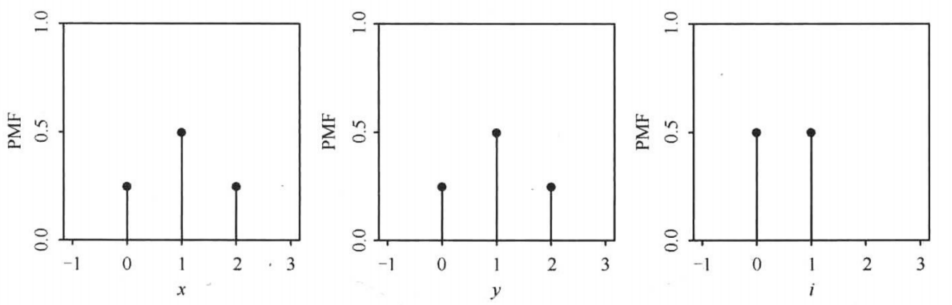
\includegraphics[width=12cm]{figures/Fig3.3.png}
	\end{figure}
\end{frame}

\begin{frame}{}
	\begin{exam}
		掷两颗骰子,其样本空间 $\Omega$ 含有 36 个等可能的样本点
		\begin{eqnarray*}
			\Omega=\{(x,y):x,y=1,2,\cdots,6\}
		\end{eqnarray*}
		令 $X$ 和 $Y$ 表示每个骰子分别出现的点数。试求下面随机变量的分布列: % 在 $\Omega$ 上定义如下三个随机变量,请给出其概率分布列
		\begin{enumerate}[<+-|alert@+>]
			\item $T_1:=X+Y=\mbox{骰子点数之和}$;
			\item $T_2:=14-(X+Y)$;
			\item $T_3:=\mbox{点数为 6 点的骰子的个数}$;
			\item $T_4:=\max\{X, Y\}=\mbox{骰子的最大点数}$
		\end{enumerate}

	\end{exam}
\end{frame}

\begin{frame}
	\begin{itemize}[<+-|alert@+>]
		\item $T_1, T_2$ 的概率分布列为 \pause
		      \begin{eqnarray*}
			      \left(\begin{array}{ccccccccccc}
				      2            & 3            & 4            & 5            & 6            & 7            & 8            & 9            & 10           & 11           & 12           \\
				      \frac{1}{36} & \frac{2}{36} & \frac{3}{36} & \frac{4}{36} & \frac{5}{36} & \frac{6}{36} & \frac{5}{36} & \frac{4}{36} & \frac{3}{36} & \frac{2}{36} & \frac{1}{36}
			      \end{array}\right)
		      \end{eqnarray*}
		      \pause
		      \begin{figure}[图 3.4.png]
			      \centering
			      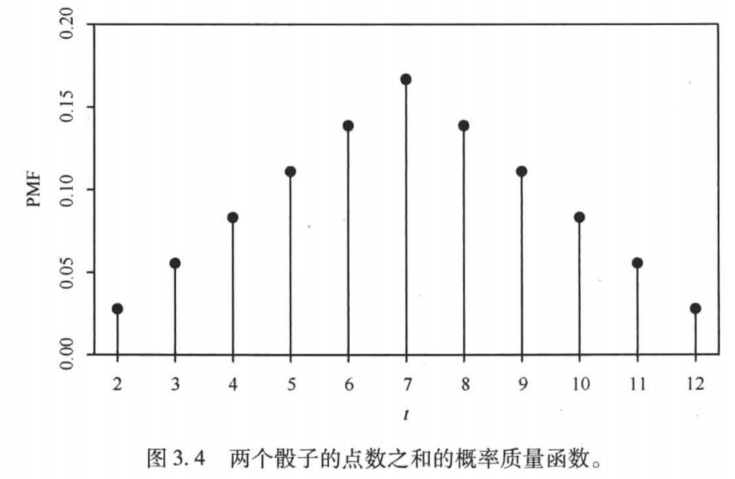
\includegraphics[width=9cm]{figures/Fig3.4.png}
		      \end{figure}

	\end{itemize}

\end{frame}

\begin{frame}
	\begin{itemize}[<+-|alert@+>]

		\item $T_3$ 的概率分布列为 \pause
		      \begin{eqnarray*}
			      \left(\begin{array}{ccc}
				      0             & 1             & 2            \\
				      \frac{25}{36} & \frac{10}{36} & \frac{1}{36}
			      \end{array}\right)
		      \end{eqnarray*}

		\item $T_4$ 的概率分布列为 \pause
		      \begin{eqnarray*}
			      \left(\begin{array}{cccccc}
				      1            & 2            & 3            & 4            & 5            & 6             \\
				      \frac{1}{36} & \frac{3}{36} & \frac{5}{36} & \frac{7}{36} & \frac{9}{36} & \frac{11}{36}
			      \end{array}\right)
		      \end{eqnarray*}
	\end{itemize}

\end{frame}

% \begin{frame}
%   \begin{exam}
%     设离散型随机变量的 $X$ 分布列为
%     \begin{eqnarray*}
%       \left(\begin{array}{ccc}
%               -1  &2 &3\\
%               0.25 & 0.5 & 0.25
%             \end{array}\right)
%     \end{eqnarray*}
%     试求 $P (X\le 0.5), P (1.5<X\le 2.5)$, 并写出 $X$ 的分布函数.
%   \end{exam}

%   \jieda $$P(X\le 0.5)=P(X=-1)=0.25,$$ $$P(1.5<X\le 2.5)=P(X=2)=0.5.$$

%   其分布函数为 \pause
%   \begin{eqnarray*}
%     F(x)=\left\{
%     \begin{array}{ll}
%       \pause  0, &  x<-1\\  \pause
%       \pause 0.25,& -1\le x<2\\  \pause
%       \pause  0.25+0.5=0.75,&  2\le x<3\\  \pause
%       \pause  0.25+0.5+0.25, & x\ge 3 \pause
%     \end{array}\right.
%   \end{eqnarray*}

% \end{frame}




\begin{frame}
	\frametitle{连续型随机变量}
	\begin{defi}[连续型随机变量] 设 $X$ 为一随机变量,$F (x)$ 为随机变量 $X$ 的分布函数,如果存在非负可积函数 $p (x)$ 使得
		\begin{eqnarray}\label{eq:contrvdist}
			F(x)=\int_{-\infty}^xp(y)dy
		\end{eqnarray}
		则称 $X$ 为连续型随机变量,其分布函数称之为连续型分布函数,函数 $p (x)$ 称为 $X$ 的概率密度函数,简称密度函数或密度.
	\end{defi}
	\pause
	\begin{rmk}
		\begin{itemize}[<+-|alert@+>]
			\item 能够表为 \eqref{eq:contrvdist} 式变上限积分的函数 $F (x)$ 在分析中称为绝对连续函数。绝对连续函数必为连续函数.
			\item 在若干个点上或零测集上改变密度函数 $p (x)$ 的值并不影响其积分的值,从而不影响分布函数 $F (x)$ 的值,这意味着连续分布的密度函数不唯一.
		\end{itemize}
	\end{rmk}

\end{frame}

\begin{frame}
	\frametitle{密度函数的性质}
	容易验证,随机变量 $X$ 的密度函数有以下性质
	\begin{enumerate}[<+-|alert@+>]
		\item 非负性:$p (x)\ge 0$;
		\item 正则性:$\int_{-\infty}^\infty p (x) dx=1$.
	\end{enumerate}

\end{frame}


\begin{frame}
	\frametitle{连续型随机变量的一些常见性质}
	\begin{itemize}
		\item $p(x)=F^\prime (x)$;
		\item $P(a< X\le b)=F(b)-F(a)=\int_a^bp(x)dx$;
		\item $0\le P (X=a)\le P (X\in (a-\epsilon,a))=\int_{a-\epsilon}^ap (x) dx\stackrel{\epsilon\rightarrow 0}{\longrightarrow} 0$, 故 $P (X=a)=0$,即连续型随机变量取值单点的概率为 0;
		\item $P(a<X\le b)=P(a\le X<b)=P(a\le X\le b)=P(a<X<b)$;
		\item 对任意的 Borel 集 $B$,
		      \begin{eqnarray*}
			      P(X\in B)=\int_Bp(x)dx
		      \end{eqnarray*}
		\item $P(X\in[x,x+\Delta x])=\int_x^{x+\Delta x}p(y)dy=p(\xi)\Delta x\approx p(x)\Delta x$
	\end{itemize}
\end{frame}
% \begin{frame}
%   \begin{exam}
%     向区间 $(0,a)$ 上任意投点,用 $X$ 表示这个点的坐标。设该点落在 $(0,a)$ 中任一小区间的概率与这个小区间的长度成正比,而与小区间的位置无关。求 $X$ 的分布函数及密度函数.
%   \end{exam}

%   \pause
%   \jieda 记 $X$ 的分布函数为 $F (x)$, 则
%   \begin{itemize}[<+-|alert@+>]
%   \item 当 $x<0$ 时,$\{X\le x\}$ 为不可能事件,故 $F (x)=P (X\le x)=0$;
%   \item 当 $x\ge a$ 时,$\{X\le x\}$ 是必然事件,故 $F (x)=P (X\le x)=1$;
%   \item 当 $x\in [0,a)$ 时, 有 $F (x)=P (X\le x)=P (0\le X\le x)=kx$, 其中 $k$ 为比例系数.
%   \item 注意到 $1=F (a)=P (0\le X\le a)=ka$, 故 $k=1/a$
%   \end{itemize}
%   \pause
%   故 $X$ 的分布函数为
%   \pause
%   \begin{eqnarray*}
%     F(x)=\left\{
%     \begin{array}{ll}
%       0,& x<0\\
%       x/a, & 0\le x<a\\
%       1,& x\ge a
%     \end{array}
%           \right.
%   \end{eqnarray*}
% \end{frame}
% \begin{frame}
%   下面我们求 $X$ 的密度函数,
%   \begin{itemize}
%   \item 当 $x<0$ 或 $x>a$ 时, $p (x)=F^\prime (x)=0$;
%   \item 当 $0<x<a$ 时,$p (x)=F^\prime (x)=1/a$;
%   \item 当 $x=0,a$ 时,$p (x)$ 可取任意值,一般就近取值为宜,不会影响概率的计算.
%   \end{itemize}
%   故 $X$ 的密度函数为
%   \begin{eqnarray*}
%     p(x)=\left\{
%     \begin{array}{ll}
%       1/a,&0<x<a,\\
%       0,&\mbox{其他}.
%     \end{array}
%           \right.
%   \end{eqnarray*}
%   其密度函数也可取为
%   \begin{eqnarray*}
%     p(x)=\left\{
%     \begin{array}{ll}
%       1/a,&0\le x\le a,\\
%       0,&\mbox{其他}.
%     \end{array}
%           \right.
%   \end{eqnarray*}

% \end{frame}

% \begin{frame}
%   \begin{exam}
%     某种型号电子元件的寿命 $X$(以小时计) 具有以下概率密度函数
%     \begin{eqnarray*}
%       p(x)=\left\{
%       \begin{array}{ll}
%         k/x^2,&x>1000,\\
%         0,&\mbox{其他}.
%       \end{array}
%             \right.
%     \end{eqnarray*}
%     其中 $k$ 为未知常数。现有一大批此种元件 (设各元件工作相互独立),问
%     \begin{enumerate}
%     \item 任取 1 只,其寿命大于 1500 小时的概率是多少?
%     \item 任取 4 只,4 只寿命都大于 1500 小时的概率是多少?
%     \item 任取 4 只,至少有一只寿命大于 1500 小时的概率是多少?
%     \item 若已知一只元件寿命大于 1500 小时,则该元件寿命大于 2000 小时的概率是多少?
%     \end{enumerate}

%   \end{exam}
% \end{frame}

\begin{frame}
	\begin{exam}
		定义函数 $F (x)$ 如下
		\begin{eqnarray*}
			F(x)=\left\{
			\begin{array}{ll}
				0,              & x< 0,      \\
				\dfrac{1+x}{2}, & 0\le x< 1, \\
				1,              & x\ge 1.
			\end{array}
			\right.
		\end{eqnarray*}
		试说明  \begin{enumerate}
			\item $F (x)$ 为分布函数;
			\item $F (x)$ 既非离散型也非连续型分布;
			\item $F (x)$ 可分解为
			      \begin{eqnarray*}
				      F(x)=\frac{1}{2}F_1(x)+\frac{1}{2}F_2(x)
			      \end{eqnarray*}
			      \pause  其中 \begin{eqnarray*}
				      F_1(x)=\left\{
				      \begin{array}{ll}
					      0, & x< 0,    \\
					      1, & x\ge 0.
				      \end{array}
				      \right.
				      \quad  F_2(x)=\left\{\begin{array}{ll}
					      0, & x<0,       \\
					      x, & 0\le x< 1, \\
					      1, & x\ge 1.
				      \end{array}
				      \right.
			      \end{eqnarray*}
		\end{enumerate}

	\end{exam}
\end{frame}


\begin{frame}
	\frametitle{勒贝格分解}
	\begin{thm}[勒贝格分解] 对任一分布函数 $F (x)$ 有如下分解
		\begin{eqnarray*}
			F(x)=c_1F_1(x)+c_2F_2(x)+c_3F_3(x),
		\end{eqnarray*}
		其中常数 $c_1,c_2,c_3\ge 0, c_1+c_2+c_3=1,$ 而 $F_1 (x),F_2 (x),F_3 (x)$ 都是分布函数,$F_1 (x)$ 为纯跳跃函数,$F_2 (x)$ 为绝对连续函数,$F_3 (x)$ 为奇异函数.
	\end{thm}
	\vspace{0.3cm}
	\pause
	\begin{itemize}[<+-|alert@+>]
		\item 上述定理中奇异函数的含义及定理的证明可参见一般的实变函数论教科书,这里我们不再详述,仅指出几种特殊情况:
		      \begin{itemize}
			      \item 在分解式中取 $c_1=1,c_2=c_3=0$ 便得到我们所讨论的离散型分布函数;
			      \item 在分解式中取 $c_2=1,c_1=c_3=0$ 便得到连续型分布函数;
			      \item 若取 $c_3=0, c_1\neq 0, c_2\neq 0, c_1+c_2=1$ 便得到离散与连续混合分布
		      \end{itemize}
		\item 从上面分析可看出,随机变量除了离散型与连续型外还有很多其他类型.
	\end{itemize}

\end{frame}


